\documentclass[11pt,a4paper]{article}
\usepackage[margin=18mm,top=18mm,bottom=20mm]{geometry}
\usepackage{fontspec}
\setmainfont{Arial}
\usepackage{tikz}
\usetikzlibrary{calc,arrows.meta,patterns,positioning,shapes.geometric}
\usepackage{xcolor,booktabs,tabularx,array,enumitem,hyperref,fancyhdr,caption,float,multicol}
\definecolor{teal}{HTML}{087F73}
\definecolor{darkteal}{HTML}{075A55}
\definecolor{green}{HTML}{2D7D46}
\definecolor{red}{HTML}{B3261E}
\definecolor{sand}{HTML}{F5D39A}
\definecolor{cyanbg}{HTML}{D8F1F0}
\definecolor{ink}{HTML}{223033}
\definecolor{muted}{HTML}{5C696C}
\definecolor{gridc}{HTML}{B7CAC8}
\hypersetup{colorlinks=true,linkcolor=darkteal,urlcolor=darkteal,pdftitle={ACC Manual}}
\pagestyle{fancy}\fancyhf{}\lhead{ACC Manual}\rhead{Wheelchair Route Checker}\cfoot{\thepage}
\setlength{\headheight}{14pt}
\setlength{\parindent}{0pt}\setlength{\parskip}{6pt}
\setlist{leftmargin=6mm,itemsep=2pt,topsep=3pt}
\newcommand{\term}[1]{\textbf{#1}}
\newcommand{\code}[1]{\texttt{#1}}
\newcommand{\stage}[1]{\par\vspace{3pt}{\color{darkteal}\bfseries\large #1}\par}
\newcommand{\smallnote}[1]{\begin{center}\fcolorbox{gridc}{cyanbg}{\parbox{0.91\linewidth}{#1}}\end{center}}
\newcommand{\door}[2]{\fill[green] (#1-0.16,#2-0.32) rectangle (#1+0.16,#2+0.32);}
\newcommand{\wheelchair}[2]{\begin{scope}[shift={(#1,#2)}]\draw[ink,line width=1.2pt] (-.25,-.18) circle (.18);\draw[ink,line width=1pt] (.26,-.2) circle (.09);\fill[blue!65!black] (-.15,.03) rectangle (.25,.25);\fill[purple!70] (-.08,.25) rectangle (.14,.47);\fill[orange!50] (.03,.58) circle (.12);\end{scope}}
\title{\vspace{35mm}\textbf{\Huge ACC Manual}\\[4mm]\Large How the Wheelchair Route Checker Works\\[8mm]\large From an IFC file to 2D plans, a 2.5D simulation, SHACL results, and an Ollama explanation}
\author{Accessibility Checking Assistant}
\date{July 2026}

\begin{document}
\maketitle
\thispagestyle{empty}
\vfill
\begin{center}
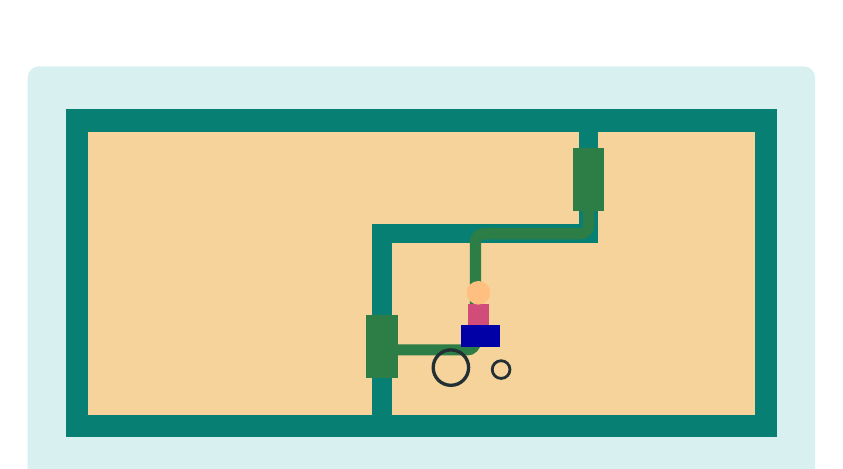
\begin{tikzpicture}[scale=1.25]
\fill[cyanbg,rounded corners=4pt] (-4,-2.1) rectangle (4,2.1);
\fill[sand] (-3.5,-1.55) rectangle (3.5,1.55);
\draw[teal,line width=8pt] (-3.5,-1.55)--(3.5,-1.55)--(3.5,1.55)--(-3.5,1.55)--cycle;
\draw[teal,line width=7pt] (-.4,-1.55)--(-.4,.4)--(1.7,.4)--(1.7,1.55);
\door{-0.4}{-0.75}\door{1.7}{0.95}
\draw[green,line width=4pt,rounded corners=3pt] (-.4,-.78)--(.55,-.78)--(.55,.4)--(1.7,.4)--(1.7,.92);
\wheelchair{.55}{-.78}
\end{tikzpicture}
\end{center}
\vfill
\smallnote{This manual describes the code that is in the project. It separates route calculation, rule checking, drawing, animation, and language generation so that each part is easy to identify.}
\newpage

\tableofcontents
\newpage

\section{The whole project in one sentence}
The program reads a digital building file, turns rooms and building parts into measurable data, finds routes between doors, checks those routes against accessibility rules, and shows the result in several views.

There is no single ``magic algorithm.'' Different jobs use different tools:
\begin{itemize}
\item \term{IfcOpenShell} reads geometry and IFC relationships.
\item \term{IFCtoLBD} converts IFC meaning into RDF triples.
\item \term{A*} finds a path across a room while avoiding blocked grid cells.
\item \term{Dijkstra's algorithm} joins door-to-door edges into shortest routes across a floor.
\item \term{SHACL} checks measurements and assigns pass/fail reasons.
\item \term{SVG} draws the 2D floor plan.
\item \term{Three.js and WebGL} draw the building model and wheelchair simulation.
\item \term{Ollama} writes a short explanation of results that already exist.
\end{itemize}

\begin{figure}[H]\centering
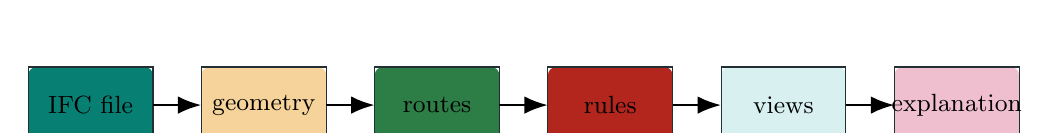
\begin{tikzpicture}[scale=.88]
\foreach \x/\label/\col in {0/IFC file/teal,2.5/geometry/sand,5/routes/green,7.5/rules/red,10/views/cyanbg,12.5/explanation/purple!25}{
  \fill[\col,rounded corners=3pt] (\x,0) rectangle +(1.8,1.1);
  \draw[ink] (\x,0) rectangle +(1.8,1.1);
  \node[align=center,font=\small] at (\x+.9,.55){\label};
}
\foreach \x in {1.8,4.3,6.8,9.3,11.8}{\draw[-{Latex[length=3mm]},line width=1pt] (\x,.55)--+(0.7,0);}
\end{tikzpicture}
\caption{The six kinds of work. This is a labelled system strip, not the route-search graph.}
\end{figure}

\section{Stage 1: Reading the IFC building}
\stage{What goes in}
An \term{IFC file} is a structured building model. It can contain walls, doors, rooms, stairs, ramps, storeys, names, identifiers, placements, and shapes. The program does not treat it as a picture. It reads objects and relationships.

\stage{What technology does the work}
\term{IfcOpenShell} opens the IFC file. Its geometry engine creates a shape for each useful object. The project calculates an axis-aligned bounding box: the smallest box, aligned with the X, Y, and Z axes, that encloses the shape. It also records the centre, size, IFC type, storey, and GlobalId.

\begin{figure}[H]\centering
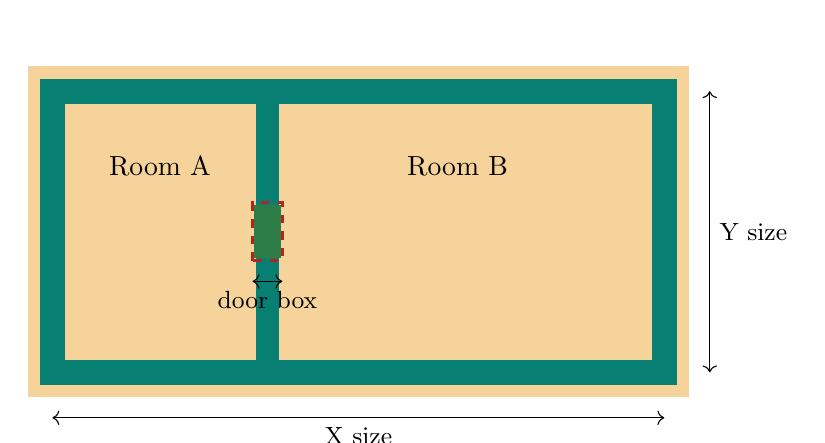
\begin{tikzpicture}[scale=1.05]
\fill[sand] (-4,-2) rectangle (4,2);
\draw[teal,line width=9pt] (-3.7,-1.7)--(3.7,-1.7)--(3.7,1.7)--(-3.7,1.7)--cycle;
\draw[teal,line width=8pt] (-1.1,-1.7)--(-1.1,1.7);
\door{-1.1}{0}
\draw[red,dashed,line width=1.2pt] (-1.28,-.35) rectangle (-.92,.35);
\draw[<->] (-1.28,-.6)--(-.92,-.6) node[midway,below,font=\small]{door box};
\draw[<->] (4.25,-1.7)--(4.25,1.7) node[midway,right,font=\small]{Y size};
\draw[<->] (-3.7,-2.25)--(3.7,-2.25) node[midway,below,font=\small]{X size};
\node at (-2.4,.8){Room A};\node at (1.2,.8){Room B};
\end{tikzpicture}
\caption{Plan-view drawing of two spaces, a wall and one door bounding box.}
\end{figure}

\stage{Why storeys matter}
Routes should connect doors on the same floor. The code compares storey data and elevation. Objects from a roof or another floor must not silently become floor obstacles. The simulation later flattens a selected floor into a floor slice, but the original geometry remains available for measurements.

\section{Stage 2: Turning IFC meaning into RDF}
Geometry says where an object is. It does not always say what that object means in a way that a rule engine can query easily. \term{IFCtoLBD 2.43.4} converts IFC information into \term{RDF}.

RDF stores small facts called \term{triples}: subject, predicate, object. For example:
\begin{center}\code{Door-18  hasStorey  GroundFloor}\end{center}

The converter is Java software. The project uses its pinned Java libraries so that the same converter version is used on another computer. The output is a Turtle file named \code{raw\_lbd\_graph.ttl}. The program parses this file with \term{RDFLib}.

\begin{figure}[H]\centering
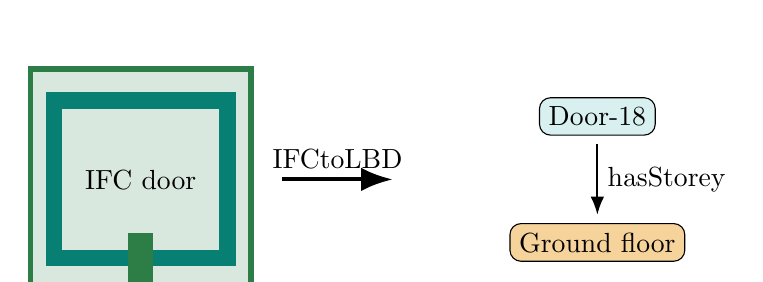
\begin{tikzpicture}[scale=1]
\fill[green!18] (-5,-1.4) rectangle (-2.2,1.4);\draw[green,line width=2pt] (-5,-1.4) rectangle (-2.2,1.4);
\draw[teal,line width=6pt] (-4.7,-1)--(-2.5,-1)--(-2.5,1)--(-4.7,1)--cycle;\door{-3.6}{-1}
\node at (-3.6,0){IFC door};
\draw[-{Latex[length=4mm]},line width=1.5pt] (-1.8,0)--(-.4,0) node[midway,above]{IFCtoLBD};
\node[draw,rounded corners,fill=cyanbg,align=center] at (2.2,.8){Door-18};
\node[draw,rounded corners,fill=sand,align=center] at (2.2,-.8){Ground floor};
\draw[-{Latex},thick] (2.2,.45)--(2.2,-.45) node[midway,right]{hasStorey};
\end{tikzpicture}
\caption{The building object remains geometry; RDF adds machine-readable meaning.}
\end{figure}

\smallnote{IFCtoLBD does not find wheelchair routes. It prepares semantic building facts. Route geometry is calculated separately by Python code.}

\begin{figure}[H]\centering
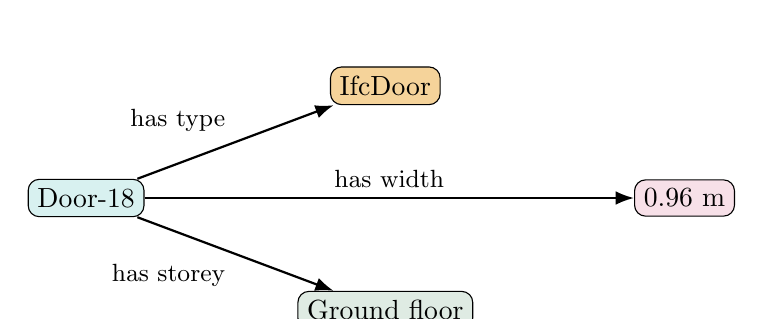
\begin{tikzpicture}[scale=.95]
\node[draw,rounded corners,fill=cyanbg] (d) at (-4,0){Door-18};
\node[draw,rounded corners,fill=sand] (t) at (0,1.5){IfcDoor};
\node[draw,rounded corners,fill=green!15] (s) at (0,-1.5){Ground floor};
\node[draw,rounded corners,fill=purple!12] (w) at (4,0){0.96 m};
\draw[-{Latex},thick] (d)--(t) node[midway,above left,font=\small]{has type};
\draw[-{Latex},thick] (d)--(s) node[midway,below left,font=\small]{has storey};
\draw[-{Latex},thick] (d)--(w) node[midway,above,font=\small]{has width};
\end{tikzpicture}
\caption{One RDF subject can connect to several facts. This is a fact drawing, not a route graph.}
\end{figure}

\section{Stage 3: Finding which doors share a space}
The route builder reads \code{IfcRelSpaceBoundary}. This IFC relationship says that an element touches or bounds a space. When a space has two or more usable doors, the program considers door pairs inside that space.

Lift doors and objects marked as unsuitable route doors are excluded. Duplicate doors are removed. The result is not yet a path. It is only a list of door pairs that may be connectable through the same room or corridor.

\begin{figure}[H]\centering
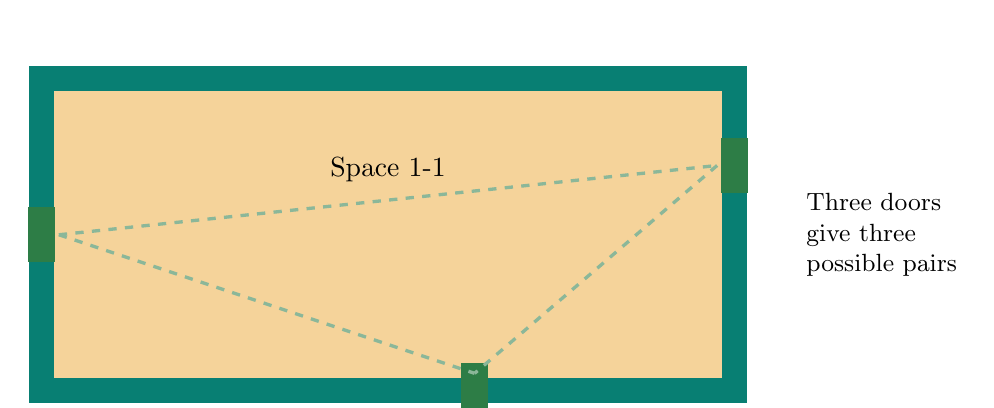
\begin{tikzpicture}[scale=1.1]
\fill[sand] (-4,-1.8) rectangle (4,1.8);\draw[teal,line width=9pt] (-4,-1.8)--(4,-1.8)--(4,1.8)--(-4,1.8)--cycle;
\door{-4}{0}\door{4}{.8}\door{1}{-1.8}
\node at (0,.75){Space 1-1};
\draw[green!55,line width=1.2pt,dashed] (-3.8,0)--(3.8,.8);
\draw[green!55,line width=1.2pt,dashed] (-3.8,0)--(1,-1.6);
\draw[green!55,line width=1.2pt,dashed] (3.8,.8)--(1,-1.6);
\node[align=left,font=\small] at (5.7,0){Three doors\\give three\\possible pairs};
\end{tikzpicture}
\caption{Candidate pairs are made only between doors that belong to the same space boundary set. Dashed lines here mean ``pair to test,'' not final routes.}
\end{figure}

\begin{figure}[H]\centering
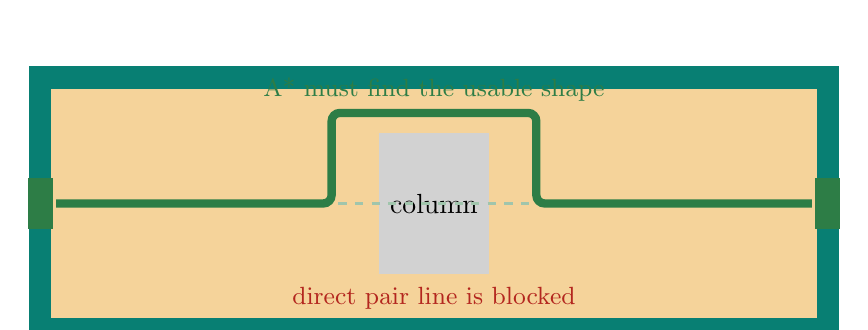
\begin{tikzpicture}[scale=1]
\fill[sand] (-5,-1.6) rectangle (5,1.6);\draw[teal,line width=8pt] (-5,-1.6)--(5,-1.6)--(5,1.6)--(-5,1.6)--cycle;
\door{-5}{0}\door{5}{0}\fill[gray!35] (-.7,-.9) rectangle (.7,.9);\node at (0,0){column};
\draw[green!45,dashed,line width=1pt] (-4.8,0)--(4.8,0);
\draw[green,line width=3pt,rounded corners=3pt] (-4.8,0)--(-1.3,0)--(-1.3,1.15)--(1.3,1.15)--(1.3,0)--(4.8,0);
\node[font=\small,red] at (0,-1.2){direct pair line is blocked};
\node[font=\small,green] at (0,1.45){A* must find the usable shape};
\end{tikzpicture}
\caption{A door pair only says what should be connected. It does not assume that the straight line is safe.}
\end{figure}

\section{Stage 4: Building two occupancy grids}
The final implementation uses two four-direction grids because it solves two different route questions.

The \term{door-route grid} is built inside each shared IFC space. Each cell represents \term{0.10 m by 0.10 m}. Preprocessing uses this grid to calculate the stored door-to-door RouteEdges. Walls, stairs, columns and other hard obstacles are marked as blocked from their IFC-derived bounding boxes. These boxes are expanded by \term{0.38 m} for the visual door-route clearance used by this project.

The \term{interactive point-route grid} covers each complete floor at \term{0.01 m by 0.01 m} resolution. It blocks walls, columns, stairs, inaccessible ramps, doors narrower than 0.90 m, and spaces narrower than the 1.50 m route-width requirement. A 0.90 m wheelchair envelope has a 0.45 m radius. After the 0.005 m geometric tolerance is applied, wall and hard-obstacle rectangles are expanded by \term{0.445 m} around the route centre.

Doors need controlled openings. The program splits wall rectangles at accessible doors and creates a portal only where the door is wide enough. This prevents a small gap beside a door from becoming a false route through the wall.

\begin{figure}[H]\centering
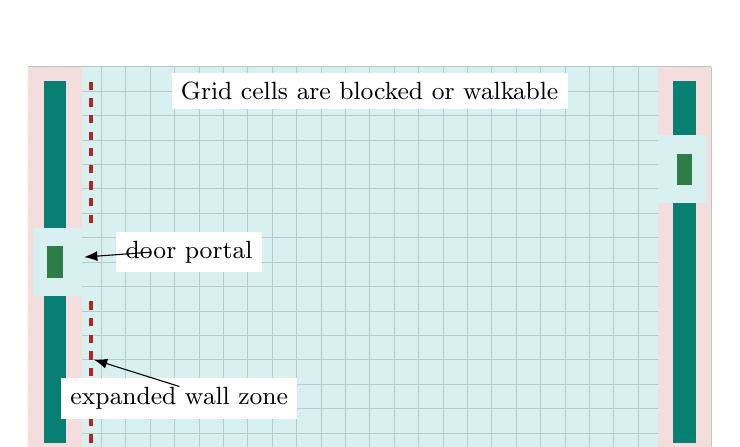
\begin{tikzpicture}[scale=.62]
\fill[cyanbg] (-7,-4) rectangle (7,4);
\draw[step=.5,gridc,very thin] (-7,-4) grid (7,4);
\fill[red!15] (-7,-4) rectangle (-5.9,4);\fill[red!15] (5.9,-4) rectangle (7,4);
\draw[teal,line width=8pt] (-6.45,-3.7)--(-6.45,3.7);\draw[teal,line width=8pt] (6.45,-3.7)--(6.45,3.7);
\fill[cyanbg] (-6.9,-.7) rectangle (-5.9,.7);\door{-6.45}{0}
\fill[cyanbg] (5.9,1.2) rectangle (6.9,2.6);\door{6.45}{1.9}
\draw[red,dashed,line width=1.5pt] (-5.7,-3.7)--(-5.7,-.8);\draw[red,dashed,line width=1.5pt] (-5.7,.8)--(-5.7,3.7);
\node[font=\small,fill=white] at (0,3.5){Grid cells are blocked or walkable};
\node[font=\small,fill=white] at (-3.9,-2.8){expanded wall zone};
\draw[-{Latex}] (-3.9,-2.55)--(-5.65,-2);
\node[font=\small,fill=white] at (-3.7,.2){door portal};\draw[-{Latex}] (-4.5,.2)--(-5.85,.1);
\end{tikzpicture}
\caption{A real occupancy-grid drawing: blocked margins remain beside the wall, while the door portal is opened.}
\end{figure}

The point-route grid is divided into \term{5 m by 5 m tiles}. Each 500 by 500 cell tile is packed into bits, compressed with zlib, and stored under \code{navigation/tiles}. The server loads only tiles needed by the selected floor and route, checks each tile's SHA-256 digest, and keeps at most 64 decoded tiles in memory.

\begin{figure}[H]\centering
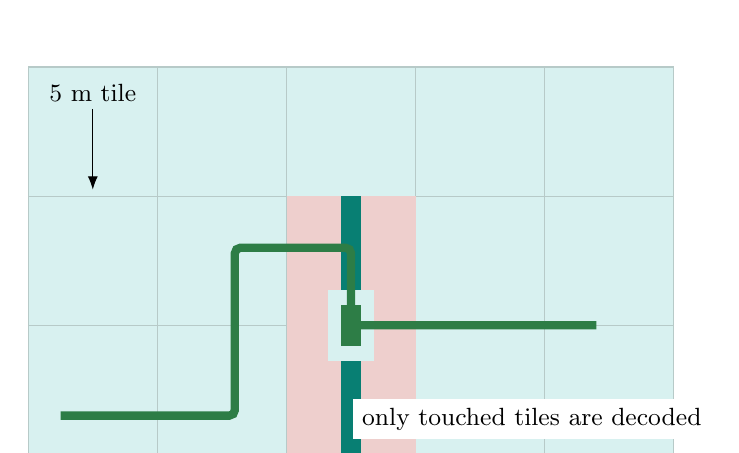
\begin{tikzpicture}[scale=.82]
\foreach \x in {0,...,4}{\foreach \y in {0,...,2}{\fill[cyanbg] (\x*2,\y*2) rectangle +(2,2);\draw[gridc] (\x*2,\y*2) rectangle +(2,2);}}
\fill[red!22] (4,0) rectangle (6,4);\draw[teal,line width=7pt] (5,0)--(5,4);
\fill[cyanbg] (4.65,1.45) rectangle (5.35,2.55);\door{5}{2}
\draw[green,line width=3pt,rounded corners=2pt] (.5,.6)--(3.2,.6)--(3.2,3.2)--(5,3.2)--(5,2)--(8.8,2);
\node[font=\small] at (1,5.6){5 m tile};\draw[-{Latex}] (1,5.35)--(1,4.1);
\node[font=\small,fill=white] at (7.8,.55){only touched tiles are decoded};
\end{tikzpicture}
\caption{The 0.01 m floor grid is streamed as 5 m tiles. The green route crosses the wall only through the accessible door portal.}
\end{figure}

\begin{figure}[H]\centering
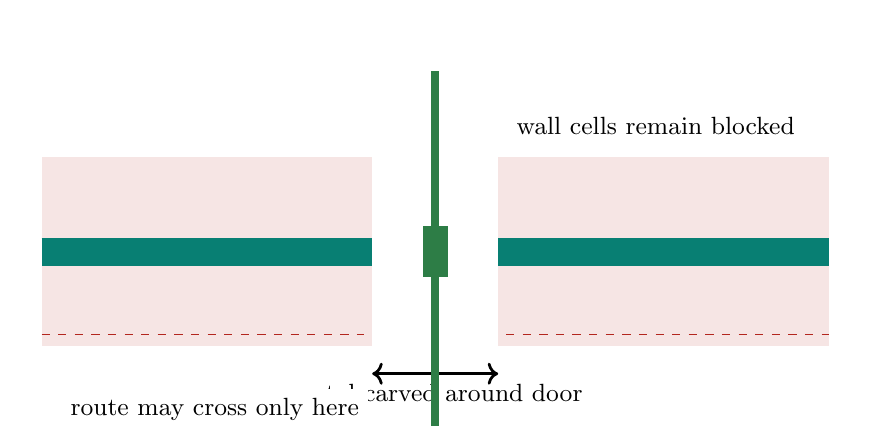
\begin{tikzpicture}[scale=1]
\fill[red!12] (-5,-1.2) rectangle (5,1.2);\draw[teal,line width=10pt] (-5,0)--(5,0);
\fill[white] (-.8,-1.2) rectangle (.8,1.2);\door{0}{0}
\draw[<->,line width=1pt] (-.8,-1.55)--(.8,-1.55) node[midway,below,font=\small]{portal carved around door};
\draw[red,dashed] (-5,-1.05)--(-.9,-1.05);\draw[red,dashed] (.9,-1.05)--(5,-1.05);
\draw[green,line width=3pt] (0,-2.3)--(0,2.3);
\node[font=\small,fill=white] at (2.8,1.6){wall cells remain blocked};
\node[font=\small,fill=white] at (-2.8,-2){route may cross only here};
\end{tikzpicture}
\caption{Close-up of a door portal. The opening is local; it does not erase the rest of the wall barrier.}
\end{figure}

\section{Stage 5: A* finds orthogonal routes}
\term{A* (A-star)} searches an occupancy grid. For a stored RouteEdge it starts at one door and tries to reach the other door. For an interactive point route it starts at the selected point and tries to reach the selected destination. Every move costs one grid step. The estimate to the target is the Manhattan distance:
\[
 h = |x-x_{target}| + |y-y_{target}|.
\]
The program permits only four moves: right, left, up, and down. Diagonal moves are absent. Therefore, grid movement is orthogonal: 0, 90, or 180 degrees.

A* chooses the cell with the smallest value of:
\[
 f = g + h,
\]
where \(g\) is the cost already travelled and \(h\) is the estimated cost still needed.

\begin{figure}[H]\centering
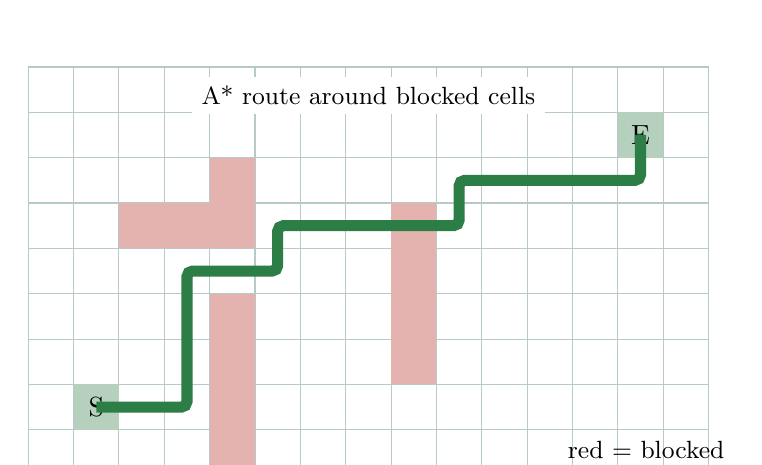
\begin{tikzpicture}[scale=.72]
\draw[step=.8,gridc] (0,0) grid (12,7.2);
\foreach \x/\y in {4/0,4/1,4/2,4/3,4/5,4/6,8/2,8/3,8/4,8/5,2/5,3/5}{\fill[red!35] (\x*.8,\y*.8) rectangle +(.8,.8);}
\fill[green!35] (.8,.8) rectangle +(0.8,.8);\node at (1.2,1.2){S};
\fill[green!35] (10.4,5.6) rectangle +(0.8,.8);\node at (10.8,6){E};
\draw[green,line width=4pt,rounded corners=2pt] (1.2,1.2)--(2.8,1.2)--(2.8,3.6)--(4.4,3.6)--(4.4,4.4)--(7.6,4.4)--(7.6,5.2)--(10.8,5.2)--(10.8,6);
\node[font=\small,fill=white] at (6,6.7){A* route around blocked cells};
\node[font=\small] at (10.9,.45){red = blocked};
\end{tikzpicture}
\caption{A* does not ``see'' the rendered wall mesh. It searches blocked and free cells derived from bounding boxes.}
\end{figure}

\begin{figure}[H]\centering
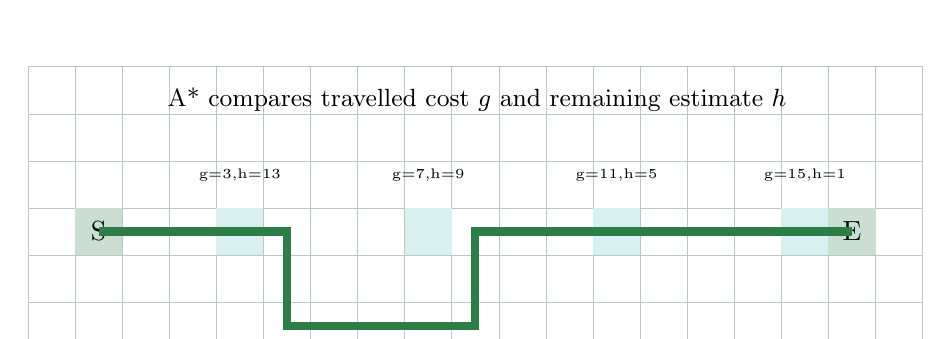
\begin{tikzpicture}[scale=.92]
\draw[step=.65,gridc,very thin] (0,0) grid (12.35,3.9);
\fill[green!25] (.65,1.3) rectangle +(0.65,.65);\node at (.975,1.625){S};
\fill[green!25] (11.05,1.3) rectangle +(0.65,.65);\node at (11.375,1.625){E};
\foreach \x/\txt in {2.6/{g=3,h=13},5.2/{g=7,h=9},7.8/{g=11,h=5},10.4/{g=15,h=1}}{
 \fill[cyanbg] (\x,1.3) rectangle +(0.65,.65);\node[font=\tiny,align=center] at (\x+.325,2.4){\txt};
}
\draw[green,line width=3pt] (.975,1.625)--(3.575,1.625)--(3.575,.325)--(6.175,.325)--(6.175,1.625)--(11.375,1.625);
\node[font=\small] at (6.2,3.45){A* compares travelled cost $g$ and remaining estimate $h$};
\end{tikzpicture}
\caption{Cost labels on selected search cells. Lower $g+h$ values are explored first.}
\end{figure}

\stage{Exact door endpoints}
Grid cells rarely sit exactly at a door centre. The code adds orthogonal endpoint connectors between the exact door centre and the first or last grid point. It then removes duplicate points, simplifies points that lie on the same straight segment, and densifies the route again.

\begin{figure}[H]\centering
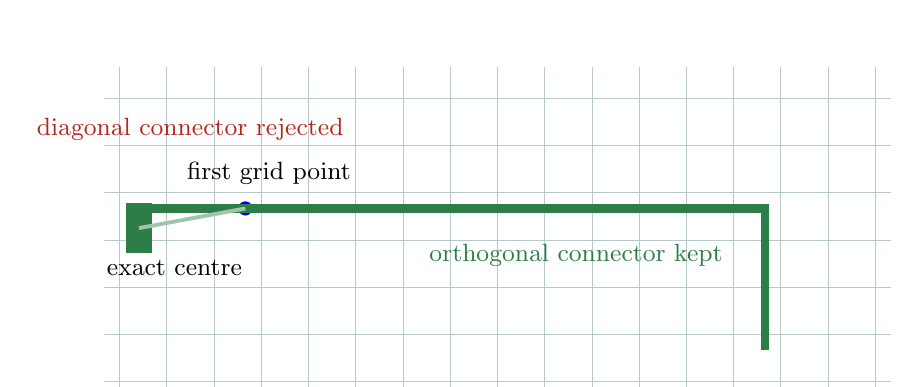
\begin{tikzpicture}[scale=1]
\draw[step=.6,gridc,very thin] (-5,-2) grid (5,2.2);
\door{-4.55}{.15}\fill[green] (-4.6,.1) circle (.09);\node[font=\small] at (-4.1,-.35){exact centre};
\fill[blue] (-3.2,.4) circle (.09);\node[font=\small] at (-2.9,.85){first grid point};
\draw[green,line width=3pt] (-4.55,.15)--(-4.55,.4)--(-3.2,.4)--(3.4,.4)--(3.4,-1.4);
\draw[green!45,line width=1.4pt] (-4.55,.15)--(-3.2,.4);
\node[font=\small,red] at (-3.9,1.4){diagonal connector rejected};
\node[font=\small,green] at (1,-.2){orthogonal connector kept};
\end{tikzpicture}
\caption{The endpoint connector starts at the actual door centre without introducing a diagonal segment.}
\end{figure}

\begin{figure}[H]\centering
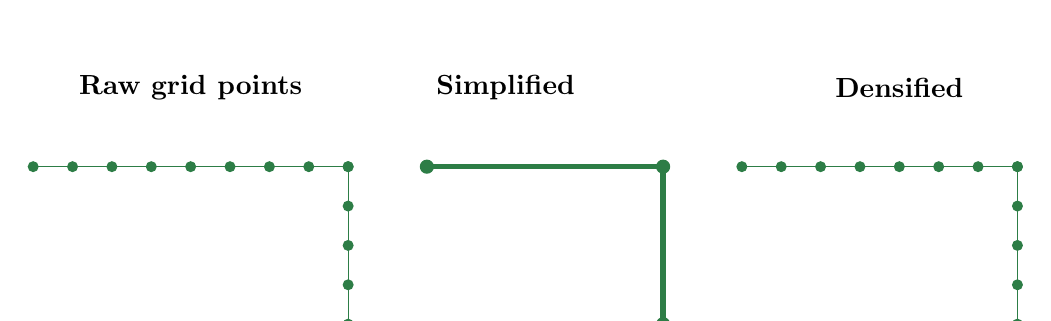
\begin{tikzpicture}[scale=1]
\node[font=\bfseries] at (-4,1.5){Raw grid points};
\foreach \x in {-6,-5.5,...,-2}{\fill[green] (\x,.5) circle (.07);}
\foreach \y in {.5,0,...,-1.5}{\fill[green] (-2,\y) circle (.07);}
\draw[green] (-6,.5)--(-2,.5)--(-2,-1.5);
\node[font=\bfseries] at (0,1.5){Simplified};
\fill[green] (-1,.5) circle (.09);\fill[green] (2,.5) circle (.09);\fill[green] (2,-1.5) circle (.09);\draw[green,line width=2pt] (-1,.5)--(2,.5)--(2,-1.5);
\node[font=\bfseries] at (5,1.5){Densified};
\foreach \x in {3,3.5,...,6.5}{\fill[green] (\x,.5) circle (.07);}
\foreach \y in {.5,0,...,-1.5}{\fill[green] (6.5,\y) circle (.07);}
\draw[green] (3,.5)--(6.5,.5)--(6.5,-1.5);
\end{tikzpicture}
\caption{Simplification stores clean corners; densification restores closely spaced checking and animation points.}
\end{figure}

\stage{The strict final check}
After construction, every dense point is checked against the occupancy grid. If the route is not clear, preprocessing stops for that pair with an error. The program does not keep a route merely because it has fewer collisions.

Interactive point routes apply the same rule when the request arrives. The backend maps both selected coordinates to stored navigation cells, loads the necessary tiles, runs four-direction A*, restores the exact clicked endpoints with orthogonal connectors, and audits the complete path. A route is green only when it reaches the requested destination, remains collision-free, and contains no diagonal segment.

If the destination is blocked or outside the accessible walking area, the backend may return a \term{red candidate}. This is not presented as an accessible route. It stays inside the start point's reachable component and ends at the last collision-free point before the obstruction. If the start itself is blocked, the result contains no path and the wheelchair Play button is disabled.

\begin{figure}[H]\centering
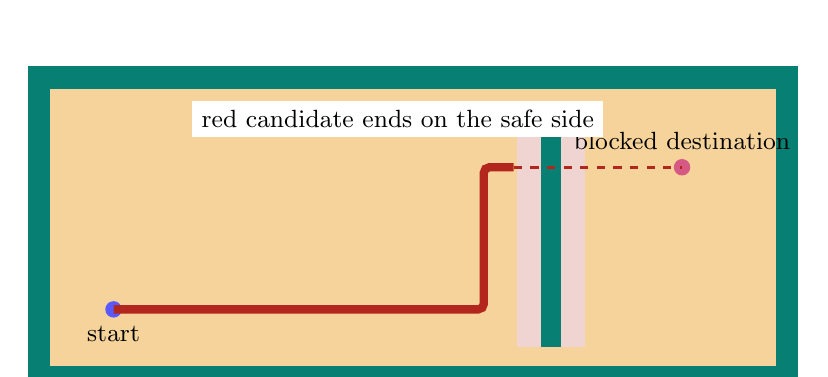
\begin{tikzpicture}[scale=.95]
\fill[sand] (-5,-2) rectangle (5,2);
\draw[teal,line width=8pt] (-5,-2)--(5,-2)--(5,2)--(-5,2)--cycle;
\fill[red!20] (1.4,-1.6) rectangle (2.3,1.6);\draw[teal,line width=7pt] (1.85,-1.6)--(1.85,1.6);
\fill[blue!65] (-4,-1.1) circle (.11);\node[font=\small,below] at (-4,-1.2){start};
\fill[purple!65] (3.6,.8) circle (.11);\node[font=\small,above] at (3.6,.9){blocked destination};
\draw[red,line width=3pt,rounded corners=2pt] (-4,-1.1)--(.95,-1.1)--(.95,.8)--(1.35,.8);
\draw[red,dashed,line width=1pt] (1.35,.8)--(3.6,.8);
\node[font=\small,fill=white] at (-.2,1.45){red candidate ends on the safe side};
\end{tikzpicture}
\caption{A blocked destination never turns a partial candidate into a green route. The dashed part is not travelled or returned as safe.}
\end{figure}

\section{Stage 6: Measuring each route edge}
Each successful A* path becomes a \term{RouteEdge}. It stores the two door IDs, a polyline, distance, measurements, status, and failure reasons.

Measurements include:
\begin{itemize}
\item minimum door width;
\item route clear width;
\item turning space when the path bends;
\item whether the route intersects a stair;
\item ramp slope and usable ramp width when applicable;
\item whether the route remains orthogonal.
\end{itemize}

\begin{figure}[H]\centering
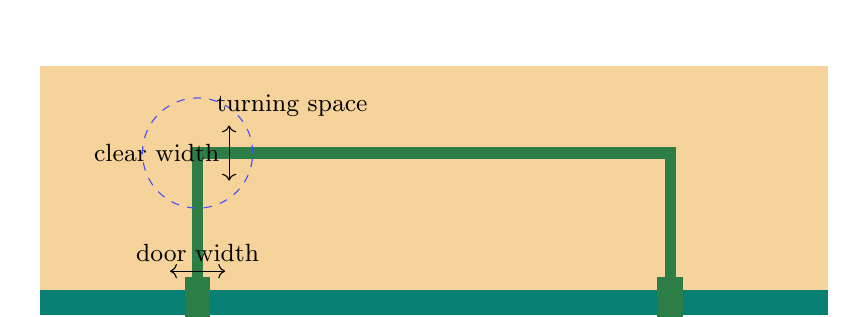
\begin{tikzpicture}[scale=1]
\fill[sand] (-5,-1.5) rectangle (5,1.5);\draw[teal,line width=9pt] (-5,-1.5)--(5,-1.5);
\door{-3}{-1.5}\door{3}{-1.5}
\draw[green,line width=4pt] (-3,-1.25)--(-3,.4)--(3,.4)--(3,-1.25);
\draw[<->] (-3.35,-1.1)--(-2.65,-1.1) node[midway,above,font=\small]{door width};
\draw[<->] (-2.6,.05)--(-2.6,.75) node[midway,left,font=\small]{clear width};
\draw[blue!70,dashed] (-3,.4) circle (.7);\node[font=\small] at (-1.8,1){turning space};
\end{tikzpicture}
\caption{Route measurements are numerical facts. The drawing is only an explanation of those facts.}
\end{figure}

\begin{figure}[H]\centering
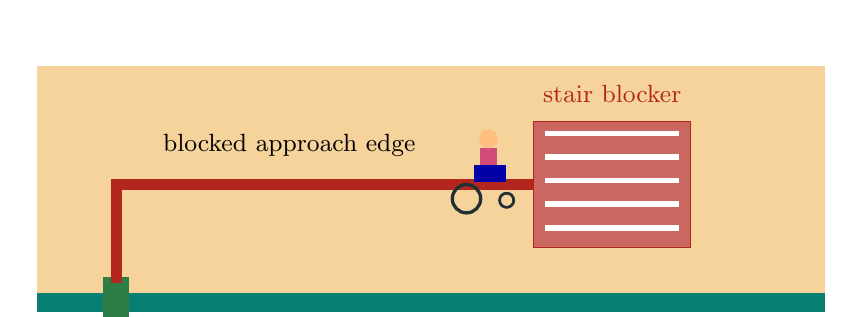
\begin{tikzpicture}[scale=1]
\fill[sand] (-5,-1.5) rectangle (5,1.5);\draw[teal,line width=7pt] (-5,-1.5)--(5,-1.5);
\draw[red,fill=red!70] (1.3,-.8) rectangle (3.3,.8);
\foreach \y in {-.55,-.25,.05,.35,.65}{\draw[white,line width=2pt] (1.45,\y)--(3.15,\y);}
\door{-4}{-1.5}\draw[red,line width=4pt] (-4,-1.25)--(-4,0)--(1.3,0);
\wheelchair{.7}{0}
\node[font=\small,red] at (2.3,1.15){stair blocker};
\node[font=\small] at (-1.8,.5){blocked approach edge};
\end{tikzpicture}
\caption{A stair-approach edge is deliberately visible and failed. The chair stops before the stair.}
\end{figure}

\stage{Special blocked stair edges}
The project also creates orthogonal approach edges from relevant doors toward stairs. These edges exist so the interface can show exactly where a wheelchair route becomes blocked by a stair. They are not successful accessible routes.

\section{Stage 7: SHACL checks the rules}
\term{SHACL} means Shapes Constraint Language. It is a rule language for RDF graphs. Python adds route measurements to the RDF graph, and \term{pySHACL} runs the shapes in \path{rules/accessibility_rules.shacl.ttl}.

SHACL checks facts such as door width, route width, turning space, stair intersection, ramp slope, and ramp width. A failed shape produces a rule identifier. The program maps that identifier to a reason such as \code{door\_width}, \code{route\_width}, \code{turning\_space}, or \code{stair\_block}.

\begin{figure}[H]\centering
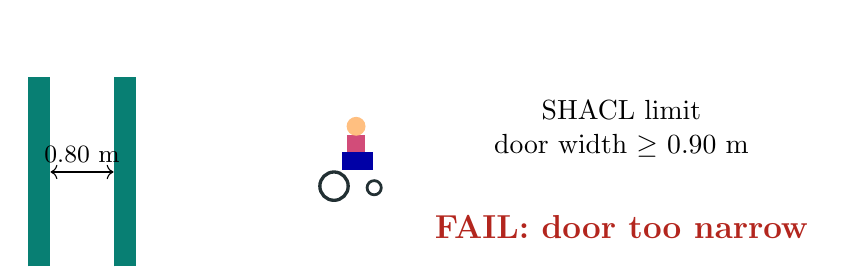
\begin{tikzpicture}[scale=1]
\draw[teal,line width=8pt] (-4,-1.2)--(-4,1.2);\draw[teal,line width=8pt] (-2.9,-1.2)--(-2.9,1.2);
\draw[<->] (-3.85,0)--(-3.05,0) node[midway,above,font=\small]{0.80 m};
\wheelchair{0}{0}
\node[align=center] at (3.4,.55){SHACL limit\\door width $\geq$ 0.90 m};
\node[red,font=\bfseries\large] at (3.4,-.7){FAIL: door too narrow};
\end{tikzpicture}
\caption{Example of a rule decision. SHACL compares stored numbers; it does not inspect pixels.}
\end{figure}

\smallnote{Ollama does not decide whether a route passes. The SHACL report and route measurements are the evidence.}

\section{Stage 8: Dijkstra joins route edges}
A* works inside one shared space and creates one edge between two doors. A floor may contain many rooms, so the program needs a second algorithm.

\term{Dijkstra's algorithm} treats doors as graph nodes and RouteEdges as graph links. The link weight is route distance in metres. Starting at a door, it repeatedly selects the nearest unreached door. This produces the shortest known route to every reachable door.

When the accessible index is built, failed edges are removed first. Dijkstra then returns only paths made from passing edges.

\begin{figure}[H]\centering
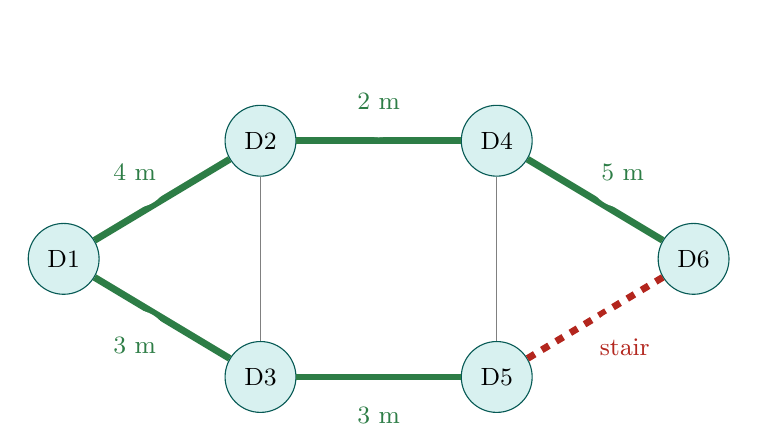
\begin{tikzpicture}[every node/.style={circle,draw=darkteal,fill=cyanbg,minimum size=9mm,font=\small},scale=1]
\node (a) at (-4,0){D1};\node (b) at (-1.5,1.5){D2};\node (c) at (-1.5,-1.5){D3};\node (d) at (1.5,1.5){D4};\node (e) at (1.5,-1.5){D5};\node (f) at (4,0){D6};
\draw[green,line width=2.5pt] (a)--(b) node[midway,above left,draw=none,fill=white]{4 m};
\draw[green,line width=2.5pt] (a)--(c) node[midway,below left,draw=none,fill=white]{3 m};
\draw[green,line width=2.5pt] (b)--(d) node[midway,above,draw=none,fill=white]{2 m};
\draw[green,line width=2.5pt] (c)--(e) node[midway,below,draw=none,fill=white]{3 m};
\draw[green,line width=2.5pt] (d)--(f) node[midway,above right,draw=none,fill=white]{5 m};
\draw[red,line width=2.5pt,dashed] (e)--(f) node[midway,below right,draw=none,fill=white]{stair};
\draw[gray] (b)--(c);\draw[gray] (d)--(e);
\end{tikzpicture}
\caption{A real door graph drawing. Dijkstra can use green passing edges. A stair-blocked edge is excluded from the accessible graph.}
\end{figure}

\begin{figure}[H]\centering
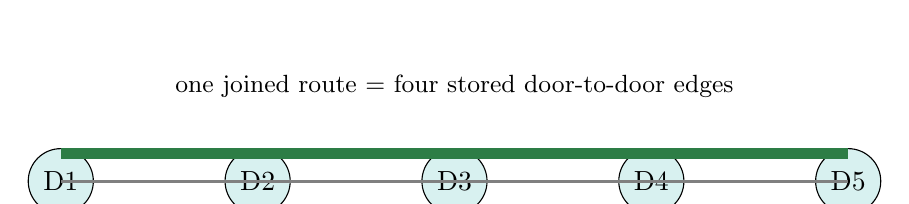
\begin{tikzpicture}[scale=1]
\foreach \x/\lab in {-5/D1,-2.5/D2,0/D3,2.5/D4,5/D5}{\node[circle,draw,fill=cyanbg,minimum size=8mm] (n\x) at (\x,0){\lab};}
\draw[gray,line width=1pt] (-5,0)--(-2.5,0)--(0,0)--(2.5,0)--(5,0);
\draw[green,line width=4pt] (-5,.35)--(-2.5,.35)--(0,.35)--(2.5,.35)--(5,.35);
\node[font=\small] at (0,1.2){one joined route = four stored door-to-door edges};
\end{tikzpicture}
\caption{The browser may animate a route made from several RouteEdge polylines joined in Dijkstra order.}
\end{figure}

\section{Stage 9: Writing the application package}
Preprocessing writes a folder that the web server can load. Important files are:
\begin{description}[style=nextline,leftmargin=8mm]
\item[\code{app\_data.json}] elements, floors, route edges, issues, routes by door, and accessible routes by door;
\item[\code{raw\_lbd\_graph.ttl}] RDF created by the pinned IFCtoLBD converter;
\item[\code{lbd\_graph.ttl}] RDF plus calculated geometry and route facts;
\item[\code{shacl\_report.ttl}] the full SHACL validation report;
\item[\code{route\_model.glb}] compact building boxes and route polylines for the building-model view;
\item[\code{route\_graph.bin}] optional fast binary copy of route edges;
\item[\code{navigation/index.json}] version, grid rules, floor bounds, tile metadata and integrity hashes;
\item[\code{navigation/tiles/*.nav}] compressed walkability tiles for interactive point routing.
\end{description}

The door graph and navigation tiles are precomputed. The browser does not rerun A* every animation frame. An interactive point request runs A* once on the precomputed 0.01 m floor cells; the resulting path is then drawn or animated.

\section{Stage 10: The Python web server}
\code{server.py} uses Python's HTTP server. It serves HTML, CSS, JavaScript, the package files, model-library data, door-route queries, point-route requests, assistant questions, project-service controls, and the Ollama restart request.

The server is also responsible for choosing a selected model package. Browser requests such as \code{/api/data} return JSON. A \code{POST /api/point-route} request contains the floor name and two IFC X/Y coordinate pairs. The deterministic backend returns the status, reason, polyline, distance, tile count and final audit. Rendering then works in the browser.

\section{Stage 11: The 2D floor plan}
The 2D plan is drawn as \term{SVG}, which means Scalable Vector Graphics. JavaScript selects elements and route edges for one floor, calculates floor bounds, and maps world X/Y positions into SVG coordinates.

Rooms, corridors, walls, doors, stairs, ramps, issues, and route polylines are separate SVG shapes. Green means passing; red means blocked. Route filtering changes what is visible, not how a stored door route was calculated.

Point-to-point mode adds two clicks to the same plan. The first click selects the start and the second selects the destination. The browser sends their IFC X/Y coordinates to the server. A green orthogonal line means the backend found and audited a complete route. A red line is only the reachable candidate: it ends at the last safe cell before the reported obstruction. The coloured dots mark the exact selected points; they do not enlarge the routing obstacles.

\begin{figure}[H]\centering
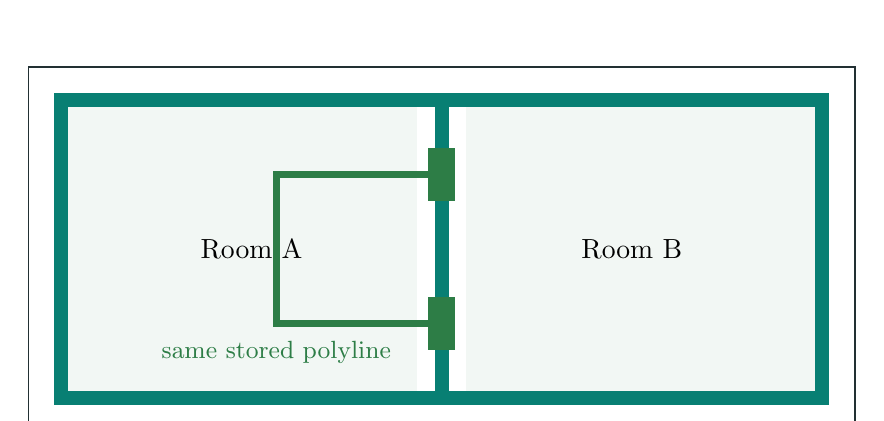
\begin{tikzpicture}[scale=1.05]
\fill[white] (-5,-2.2) rectangle (5,2.2);\draw[ink] (-5,-2.2) rectangle (5,2.2);
\fill[green!6] (-4.6,-1.8) rectangle (-.3,1.8);\fill[green!6] (.3,-1.8) rectangle (4.6,1.8);
\draw[teal,line width=5pt] (-4.6,-1.8)--(4.6,-1.8)--(4.6,1.8)--(-4.6,1.8)--cycle;\draw[teal,line width=5pt] (0,-1.8)--(0,1.8);
\door{0}{-.9}\door{0}{.9}
\draw[green,line width=2.5pt] (0,-.9)--(-2,-.9)--(-2,.9)--(0,.9);
\node at (-2.3,0){Room A};\node at (2.3,0){Room B};
\node[font=\small,green] at (-2,-1.25){same stored polyline};
\end{tikzpicture}
\caption{The 2D view projects a route onto a flat SVG plan.}
\end{figure}

\begin{figure}[H]\centering
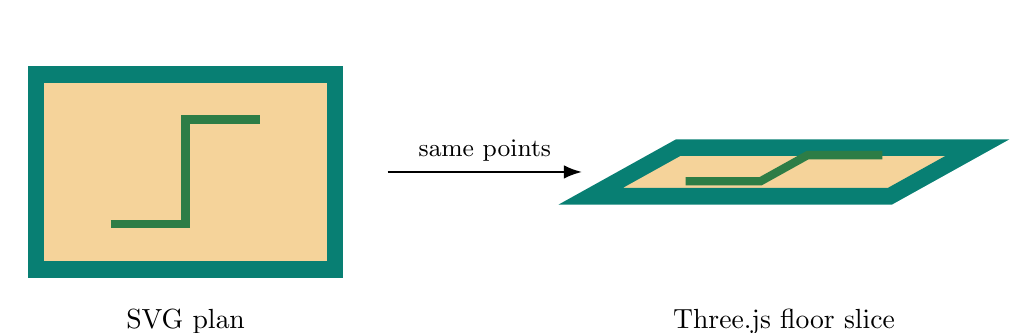
\begin{tikzpicture}[scale=.95]
\begin{scope}[shift={(-4,0)}]
\fill[sand] (-2,-1.3) rectangle (2,1.3);\draw[teal,line width=6pt] (-2,-1.3)--(2,-1.3)--(2,1.3)--(-2,1.3)--cycle;\draw[green,line width=3pt] (-1,-.7)--(0,-.7)--(0,.7)--(1,.7);\node at (0,-2){SVG plan};
\end{scope}
\draw[-{Latex},thick] (-1.3,0)--(1.3,0) node[midway,above,font=\small]{same points};
\begin{scope}[shift={(4,0)},x={(1cm,0)},y={(.45cm,.25cm)},z={(0cm,1cm)}]
\fill[sand] (-2,-1.3,0)--(2,-1.3,0)--(2,1.3,0)--(-2,1.3,0)--cycle;\draw[teal,line width=6pt] (-2,-1.3,0)--(2,-1.3,0)--(2,1.3,0)--(-2,1.3,0)--cycle;\draw[green,line width=3pt] (-1,-.7,.05)--(0,-.7,.05)--(0,.7,.05)--(1,.7,.05);
\end{scope}\node at (4,-2){Three.js floor slice};
\end{tikzpicture}
\caption{The 2D and simulation views use the same route response and draw its coordinates differently.}
\end{figure}

\section{Stage 12: The building-model view}
The building-model tab uses \term{Three.js}, a JavaScript 3D library, and \term{WebGL}, the browser's graphics system. \term{GLTFLoader} loads \code{route\_model.glb}. A perspective camera, lights, edge lines, door markers, ray casting, and orbit controls make the model inspectable.

This view is for examining the package. It is not the place where A* runs. Selecting a door asks the server for routes and draws stored route lines above the model.

\section{Stage 13: The wheelchair simulation is 2.5D}
The simulation uses 3D meshes, lighting, shadows and a camera, but it intentionally presents one flat floor slice. That is why \term{2.5D} is the most accurate name.

For the selected floor, JavaScript builds boxes for walls, doors and blockers. It uses one uniform scale and the same floor transform for every element and every route point. The X/Y route coordinates become the horizontal X/Z scene coordinates. Route height becomes one explicit floor-surface height.

\begin{figure}[H]\centering

\begin{tikzpicture}[x={(1cm,0cm)},y={(.55cm,.28cm)},z={(0cm,1cm)},scale=.9]
\fill[cyanbg] (-5,-2,0) -- (5,-2,0) -- (5,2,0) -- (-5,2,0) -- cycle;
\fill[sand] (-4,-1.5,0) -- (4,-1.5,0) -- (4,1.5,0) -- (-4,1.5,0) -- cycle;
\draw[teal,line width=7pt] (-4,-1.5,0)--(4,-1.5,0)--(4,1.5,0)--(-4,1.5,0)--cycle;
\draw[teal,line width=7pt] (0,-1.5,0)--(0,.4,0)--(2,.4,0)--(2,1.5,0);
\draw[green,line width=3.5pt] (-3,-1,0.06)--(-1,-1,0.06)--(-1,.4,0.06)--(2,.4,0.06)--(2,1,0.06);
\node at (-1,-1,0.8){wheelchair};
\draw[-{Latex}] (-1,-1,0.65)--(-1,-1,0.12);
\end{tikzpicture}
\caption{A cutaway drawing of the 2.5D floor slice. Geometry and route share one transform and one floor level.}
\end{figure}

\begin{figure}[H]\centering
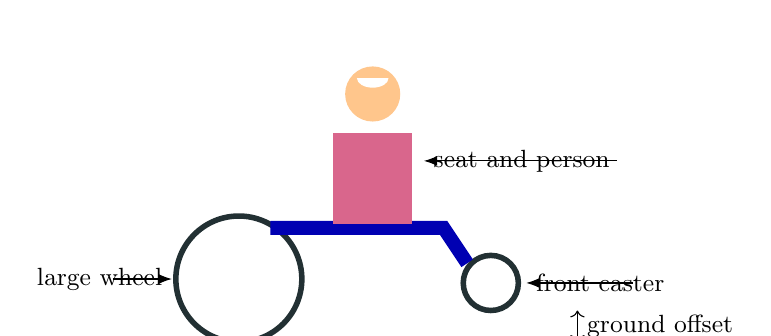
\begin{tikzpicture}[scale=1]
\draw[ink,line width=2pt] (-2,-.4) circle (.8);\draw[ink,line width=2pt] (1.2,-.45) circle (.35);
\draw[blue!70!black,line width=5pt] (-1.6,.25)--(.6,.25)--(.9,-.2);\fill[purple!60] (-.8,.3) rectangle (.2,1.45);\fill[orange!45] (-.3,1.95) circle (.35);\fill[white] (-.5,2.15) arc (180:360:.2 and .12);
\draw[-{Latex}] (-3.6,-.4)--(-2.85,-.4) node[left,font=\small]{large wheel};
\draw[-{Latex}] (3,-.45)--(1.65,-.45) node[right,font=\small]{front caster};
\draw[-{Latex}] (2.8,1.1)--(.35,1.1) node[right,font=\small]{seat and person};
\draw[red,dashed] (-3,-1.2)--(2,-1.2);\draw[<->] (2.3,-1.2)--(2.3,-.8) node[midway,right,font=\small]{ground offset};
\end{tikzpicture}
\caption{The wheelchair sprite is assembled from 3D primitives. Its lowest mesh point is placed on the floor surface.}
\end{figure}

\begin{figure}[H]\centering
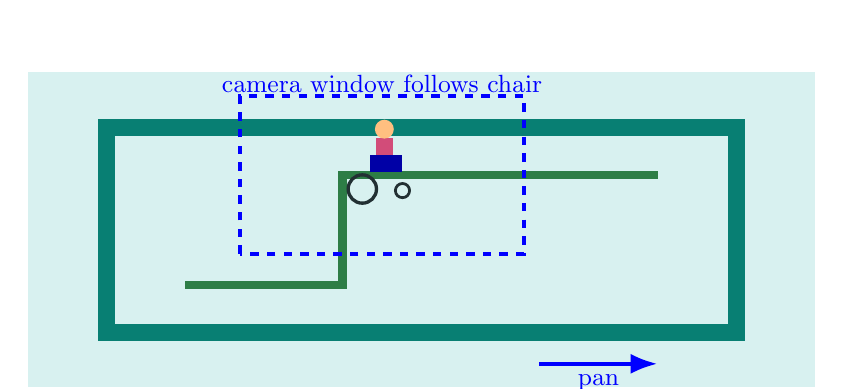
\begin{tikzpicture}[scale=1]
\fill[cyanbg] (-5,-2) rectangle (5,2);\draw[teal,line width=6pt] (-4,-1.3)--(4,-1.3)--(4,1.3)--(-4,1.3)--cycle;
\draw[green,line width=3pt] (-3,-.7)--(-1,-.7)--(-1,.7)--(3,.7);\wheelchair{-.5}{.7}
\draw[blue,dashed,line width=1.5pt] (-2.3,-.3) rectangle (1.3,1.7);\node[blue,font=\small] at (-.5,1.85){camera window follows chair};
\draw[-{Latex},blue,line width=1.5pt] (1.5,-1.7)--(3,-1.7) node[midway,below,font=\small]{pan};
\end{tikzpicture}
\caption{Panning moves the camera view. It does not move walls, change route coordinates, or rerun A*.}
\end{figure}

\stage{Animation}
The chair is built from Three.js primitives: torus wheels, boxes, cylinders and spheres. The program calculates its lowest mesh point so the tyres touch the floor. During animation, it interpolates along the stored polyline and turns the chair toward the next point.

For a failed stored stair edge, the chair stops at the configured blocked point, waits briefly, and then advances to the next route. In point-to-point mode, a clear route makes one complete pass from the selected start to the selected destination. A blocked request uses the red reachable candidate and stops at its final safe point. If the selected start itself is blocked, there is no safe candidate to animate. This movement is presentation logic. It does not change the deterministic route result or the SHACL result.

The thin lines are the other stored floor RouteEdges. They provide context. The thick green or red line is the current animated route.

\begin{figure}[H]\centering
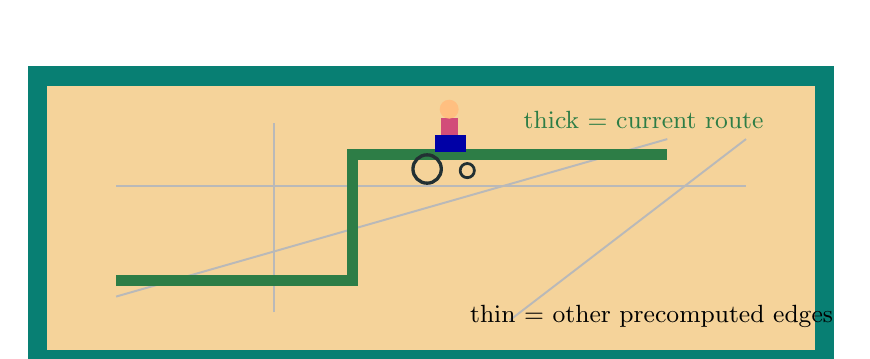
\begin{tikzpicture}[scale=1]
\fill[sand] (-5,-1.8) rectangle (5,1.8);\draw[teal,line width=7pt] (-5,-1.8)--(5,-1.8)--(5,1.8)--(-5,1.8)--cycle;
\draw[gray!55,line width=.7pt] (-4,-1)--(3,1);\draw[gray!55,line width=.7pt] (-4,.4)--(4,.4);\draw[gray!55,line width=.7pt] (-2,-1.2)--(-2,1.2);\draw[gray!55,line width=.7pt] (1,-1.3)--(4,1);
\draw[green,line width=4pt] (-4,-.8)--(-1,-.8)--(-1,.8)--(3,.8);\wheelchair{.2}{.8}
\node[font=\small] at (2.8,-1.25){thin = other precomputed edges};\node[font=\small,green] at (2.7,1.25){thick = current route};
\end{tikzpicture}
\caption{Route-line meaning in the wheelchair simulation.}
\end{figure}

\section{Stage 14: Ollama explains; it does not judge}
The Check Results page can send a question and a small block of validated facts to a local Ollama model. The model writes a short explanation. The default preferred model is \code{qwen3:8b} when installed.

The prompt tells the model to use only detected issue types, affected elements, failed routes, and floors with failures. Point-to-point explanations receive a separate structured fact set containing the selected coordinates, deterministic status, reason, distance, width and audit result. Ollama may reword those facts, but it cannot change a blocked result to clear, invent an elevator or ramp, or replace the backend reason. If Ollama is unavailable, the application returns a deterministic explanation from the same checked data.

The Restart Ollama button is maintenance code. It checks port 11434, refuses to kill an unrelated process, stops installed Ollama processes, starts one clean service, waits for the API, and warms the selected model.

\begin{figure}[H]\centering
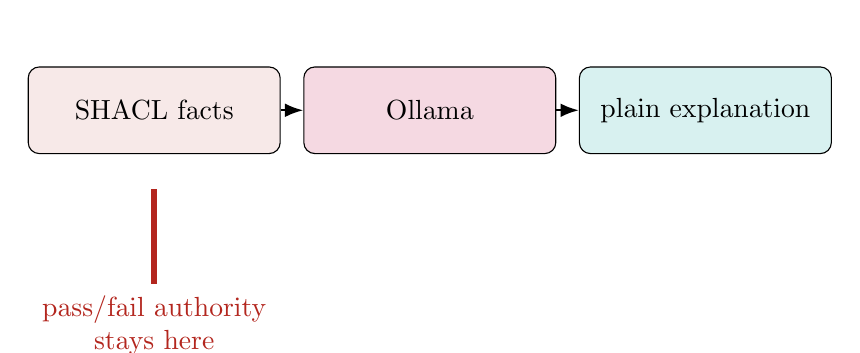
\begin{tikzpicture}[scale=1]
\node[draw,rounded corners,fill=red!10,minimum width=3.2cm,minimum height=1.1cm] (facts) at (-3.5,0){SHACL facts};
\node[draw,rounded corners,fill=purple!15,minimum width=3.2cm,minimum height=1.1cm] (ollama) at (0,0){Ollama};
\node[draw,rounded corners,fill=cyanbg,minimum width=3.2cm,minimum height=1.1cm] (words) at (3.5,0){plain explanation};
\draw[-{Latex},thick] (facts)--(ollama);\draw[-{Latex},thick] (ollama)--(words);
\draw[red,line width=2pt] (-3.5,-1)--(-3.5,-2.2) node[below,align=center]{pass/fail authority\\stays here};
\end{tikzpicture}
\caption{The language model changes wording, not route geometry or compliance status.}
\end{figure}

\section{Which part answers which question?}
\begin{tabularx}{\textwidth}{>{\bfseries}p{35mm}X X}
\toprule
Question & Responsible part & Not responsible \\
\midrule
Where are the walls and doors? & IfcOpenShell geometry and bounding boxes & Ollama \\
What touches a space? & IFC relationships, especially IfcRelSpaceBoundary & SVG \\
How does a stored door path cross a room? & Four-direction A* on the 0.10 m door grid & Three.js \\
How is a clicked point route found? & Four-direction A* on precomputed 0.01 m navigation tiles & Ollama \\
What is the shortest multi-room route? & Dijkstra over the door graph & SHACL \\
Does a route pass a rule? & SHACL over RDF measurements & The route colour itself \\
How is the 2D plan drawn? & SVG and JavaScript & A new route search \\
How is the wheelchair scene drawn? & Three.js/WebGL floor-slice rendering & IFCtoLBD \\
Who writes the explanation? & Ollama, using checked facts & A* \\
\bottomrule
\end{tabularx}

\section{Important limits}
\begin{itemize}
\item Bounding boxes are simpler than exact meshes. They are suitable for this visual route checker, but they approximate rotated or irregular shapes.
\item Stored door routes use a 0.10 m grid. Interactive point routes use 0.01 m cells stored in compressed 5 m tiles. The finer grid improves click precision but needs more preprocessing, disk space and search work.
\item The point grid expands solid obstacles by 0.445 m around the route centre. This represents a 0.90 m wheelchair envelope while retaining a 0.005 m geometry tolerance.
\item The simulation is a floor-slice presentation, not a physics engine or a certified 1:1 wheelchair test.
\item A clear route means it passed the encoded measurements and SHACL rules. It does not replace professional accessibility review or local legal approval.
\item Poor IFC relationships or missing geometry can limit what the program can calculate. The audit reports missing geometry instead of inventing it.
\end{itemize}

\section{Source map for technical readers}
\scriptsize\begin{tabularx}{\textwidth}{>{\ttfamily}p{40mm}X}
\toprule
File & Main responsibility \\
\midrule
preprocess.py & runs the complete preprocessing job \\
backend/geometry.py & extracts IFC geometry and element metadata \\
backend/ifc\_tools.py & runs the pinned IFCtoLBD Java converter \\
backend/routes.py & space boundaries, grid, A*, measurements, Dijkstra \\
backend/navigation.py & 0.01 m floor tiles, point-route A*, candidate path and final audit \\
backend/shacl\_runner.py & runs pySHACL and maps rule results \\
backend/package\_writer.py & writes browser-ready JSON and indexes \\
backend/glb\_export.py & writes the compact GLB building model \\
backend/short\_explainer.py & sends checked facts to Ollama \\
server.py & serves files and APIs; manages point requests, Ollama and verified project services \\
frontend/app.js & 2D SVG, Three.js views, point selection, simulation and controls \\
rules/ SHACL file & accessibility SHACL constraints \\
\bottomrule
\end{tabularx}
\normalsize

\section{Short recap}
The route itself begins with IFC geometry, not with Ollama. Preprocessing builds stored door routes and compressed point-navigation tiles. A* finds orthogonal paths: between doors on the 0.10 m grid, or between two selected points on the 0.01 m tiles. Dijkstra joins passing door edges into shortest routes across the door graph. SHACL checks the stored measurements. The browser draws the backend coordinates in 2D and 2.5D, and the wheelchair follows the same point-route response. Ollama explains checked facts only after the deterministic calculation is complete.

\vfill
\begin{center}\color{muted}\small ACC Manual - Accessibility Checking Assistant - July 2026\end{center}
\end{document}
